\documentclass{article}
\usepackage[danish]{babel}
\usepackage{graphicx}
\usepackage{outlines}
\usepackage{amssymb}
\usepackage{enumitem}
\usepackage{listings}
\usepackage{tabularx}
\usepackage{multirow}
\usepackage{listings}
\usepackage[T1]{fontenc}
\usepackage{inconsolata}
\usepackage{color}
\usepackage{hyperref}
\renewcommand{\labelitemi}{$\bullet$}
\renewcommand{\labelitemii}{$\circ$}
\renewcommand{\labelitemiii}{$\blacksquare$}
\renewcommand{\labelitemiv}{$\star$}
\definecolor{pblue}{rgb}{0.13,0.13,1}
\definecolor{pgreen}{rgb}{0,0.5,0}
\definecolor{pred}{rgb}{0.9,0,0}
\definecolor{pgrey}{rgb}{0.46,0.45,0.48}
\lstset{language=Java,
  showspaces=false,
  showtabs=false,
  breaklines=true,
  showstringspaces=false,
  breakatwhitespace=true,
  commentstyle=\color{pgreen},
  keywordstyle=\color{pblue},
  stringstyle=\color{pred},
  basicstyle=\ttfamily,
  moredelim=[il][\textcolor{pgrey}]{$$},
  moredelim=[is][\textcolor{pgrey}]{\%\%}{\%\%}
}
\title{%
Assignment 3 \\
\large Code optimization and reporting
}
\author{Mads Wulff Nielsen \\
Claus Kramath}
\begin{document}
\maketitle
\thispagestyle{empty}
\newpage
\tableofcontents
\thispagestyle{empty} 
\newpage
\section{Introduktion}
\paragraph{}
Programmet, vi vil forsøge at optimere, beregner frekvensen af forekomsten af et bogstav i en tekst. Programmet er klonet fra flg. github repository: 
\begin{enumerate}
    \item \url{https://github.com/CPHBusinessSoftUFO/letterfrequencies}
\end{enumerate}
Det oprindelige program indlæser en tekstfil, gennemløber karaktererne i denne enkeltvis og akkumulerer antallet af hver karakters forekomster løbende i et HashMap. Til sidst udskrives antallet af hver karakters forekomst; frekvensen.
\section{Instruktion}
\paragraph{}
Herunder er instruktioner til at køre den optimerede kode på egen maskine:
\begin{enumerate}
    \item Vores optimerede løsning kan downloades her: \\ \url{https://github.com/CK2800/UFO/tree/master/3}
    \item Åbn projektet i IntelliJ eller tilsvarende IDE.
    \item Kør Main.main() fra IDE'et, bemærk at der køres 500 loops. Vores benchmark indikerer, at det bør tage ca. 75 sek. på en i5, 2.2 GHz.
    \item Observer mean og standard deviation udregningerne i konsollen. Disse udregnes for hvert 50. loop.
    \item Kør nu Main i kommandoprompten ved at navigere til /target/classes og skrive flg. kommando:
    \begin{verbatim}
        java cphbusiness.ufo.letterfrequencies.Main
    \end{verbatim}
    
    \item Observer igen mean og standard deviation værdierne i konsollen.
\end{enumerate}
\newpage
\section{Fremgangsmåde}
\paragraph{}
For at identificere flaskehalse i programmet, har vi brugt Java flight recorder profileren, som findes i vores IDE; IntelliJ. 
Af billedet herunder fremgår det, at kørslen af programmet i sin helhed især bruger tid på \begin{verbatim}
    Main.tallyChars(Reader, Map)
\end{verbatim}
\begin{figure}[htb]
    \centering
    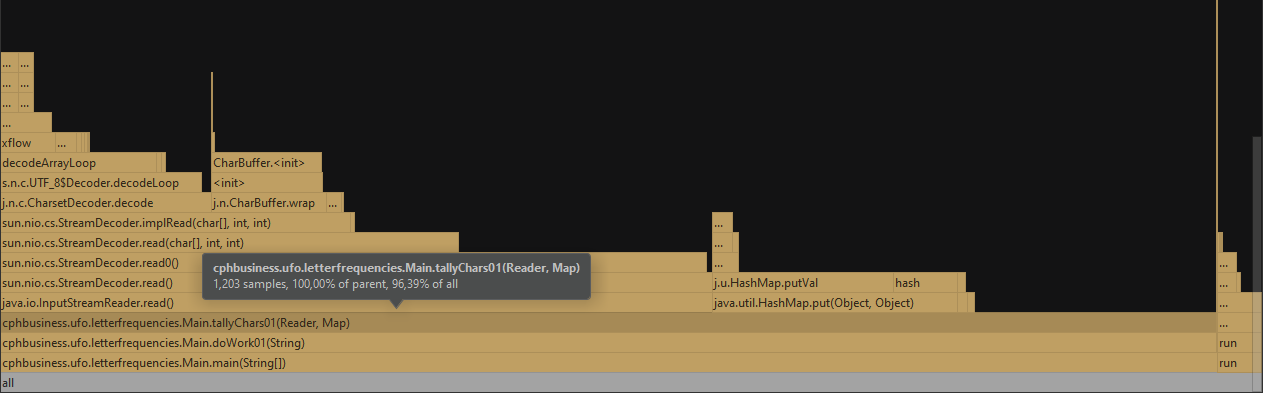
\includegraphics[width=\textwidth]{images/tallyChars01.PNG}
    \caption{Flammegraf for original tallyChars metode.}
    \label{fig:1}
\end{figure}
Billedet med flammegrafen viser også, at der er relativt mange skridt forbundet med den originale kode. Eksempelvis kaldes der ofte metoder på StreamDecoder- og CharsetDecoder-objekter, før karakteren indsættes i HashMap.
Med identifikationen af den mulige flaskehals, granskede vi den originale kode for at forstå den, samt fremkomme med umiddelbare optimeringsskridt.
\begin{figure}[htb]
    \centering
    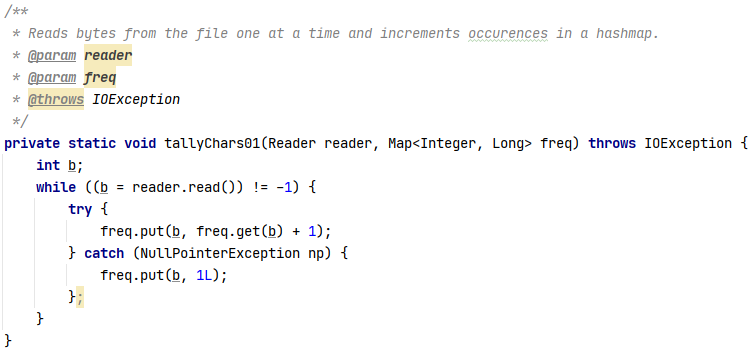
\includegraphics[width=\textwidth]{images/tallyChars01_code.PNG}
    \caption{Original tallyChars metode.}
    \label{fig:2}
\end{figure}
\paragraph{}
Vores umiddelbare mistanke faldt på det faktum, at koden traverserer hele filen, 1 bogstav ad gangen. Dette resulterer i mange læsninger på disken, hvorfor vi drøftede følgende løsningsforslag:
\begin{enumerate}
    \item Indlæsning af (dele af) filen til RAM.
    \item Anvendelse af alternativ reader, eventuelt med indbygget buffer.
    \item Læse filen i større bidder ved brug af byte arrays.
\end{enumerate}
\subsection{Fravalg af forslag 1}
\paragraph{}Vi indså hurtigt at indlæsning af filen inden kørslen af Main.tallyChars ville bryde med kontrakten, idet en ændring af indlæsningstidspunkt for filen vil medføre, at indlæsningsmetoden skal køres først. Dette vil medføre ændringer i kodebasen andre steder, idet en ny metode til indlæsning af filen i RAM ville skulle kaldes først.
\subsection{Anvendelse af alternativ reader}
\paragraph{}Med vores mistanke om flaskehalsens årsag in mente, tog vi en BufferedInputStream i brug, for at teste, om læsning af buffer fra memory ville gøre nogen forskel. Som det kan ses af flg. graf, var det en forbedring i kørselstiderne. Brugen af BufferedInputStream er imidlertid også et brud på kontrakten, idet der fordres en ny signatur på metoden:
\begin{verbatim}
    private static void tallyChars(BufferedInputStream stream, 
        Map<Integer, Long> freq)
\end{verbatim}
Anvendelsen af BufferedInputStream skal således ses som en afprøvning af konceptet med en buffer at læse fra. Senere kunne vi formentlig have brugt BufferedReader for overholdelse af kontrakten;
\begin{verbatim}
    private static void tallyChars(Reader reader, Map<Integer, 
        Long> freq)
\end{verbatim}
Som det fremgår af figurerne \ref{fig:3} - \ref{fig:6}, er indlæsning i større bidder en plausibel løsning, idet den blå kasse med hale viser den originale tallyChars-metode. Den grå kasse med hale viser tider med indlæsning vha. BufferedInputStream:
\pagebreak
\subsection{Indlæsningstider}
    \begin{figure}[htb]
        \begin{minipage}[t]{.5\textwidth}
            \centering
            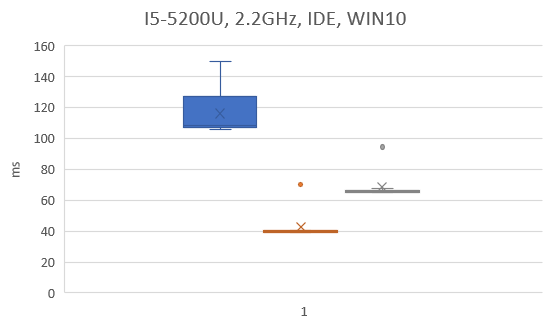
\includegraphics[width=\textwidth]{images/win10idekmh.PNG}
            \caption{Kørselstider, IDE, Win10.}\label{fig:3}
        \end{minipage}
        \hfill
        \begin{minipage}[t]{.5\textwidth}
            \centering
            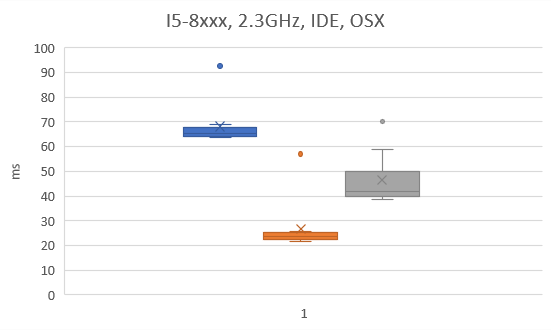
\includegraphics[width=\textwidth]{images/osxidekmh.PNG}
            \caption{Kørselstider, IDE, OSX.}\label{fig:4}
        \end{minipage}
        \hfill
        \begin{minipage}[t]{.5\textwidth}
            \centering
            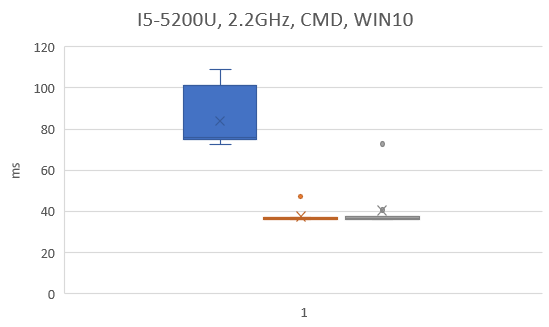
\includegraphics[width=\textwidth]{images/win10cmdkmh.PNG}
            \caption{Kørselstider, CMD, Win10.}\label{fig:5}
        \end{minipage}
        \hfill
        \begin{minipage}[t]{.5\textwidth}
            \centering
            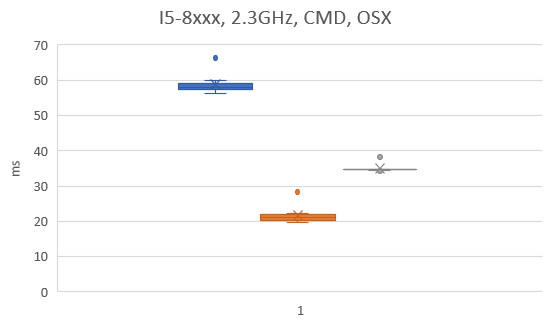
\includegraphics[width=\textwidth]{images/osxcmdkmh.PNG}
            \caption{Kørselstider, CMD, OSX.}\label{fig:6}
        \end{minipage}
    \end{figure}
\subsection{Indlæsning af filen i bidder vha. char array}
\paragraph{}Som det videre fremgår af figurerne \ref*{fig:3}-\ref*{fig:6} ovenfor, er indlæsning vha. et char-array en hurtig løsning. Den orange kasse med hale er, i alle 4 figurer, den hurtigste og har samtidig ganske stabile kørselstider, uanset om den afvikles fra ide eller kommandoprompt.
Vi har forsøgt at justere på længden af char-array'et, den bedste performance opnås dog ved enten 128 eller 256 pladser. Vores tese er, at det lagrede array, ved mange elementer, fylder mere end der er plads til i RAM, derfor skrives dele af array'et måske til disken. 
\newpage
\section{Videre optimering}
\paragraph{}
Vores optimerede kodes hurtigere kørselstid kan også ses af nedenstående flammegraf, der viser en markant mindre dybde i nestede kald fra tallyChars-metoden.
\begin{figure}[htb]
    \centering
    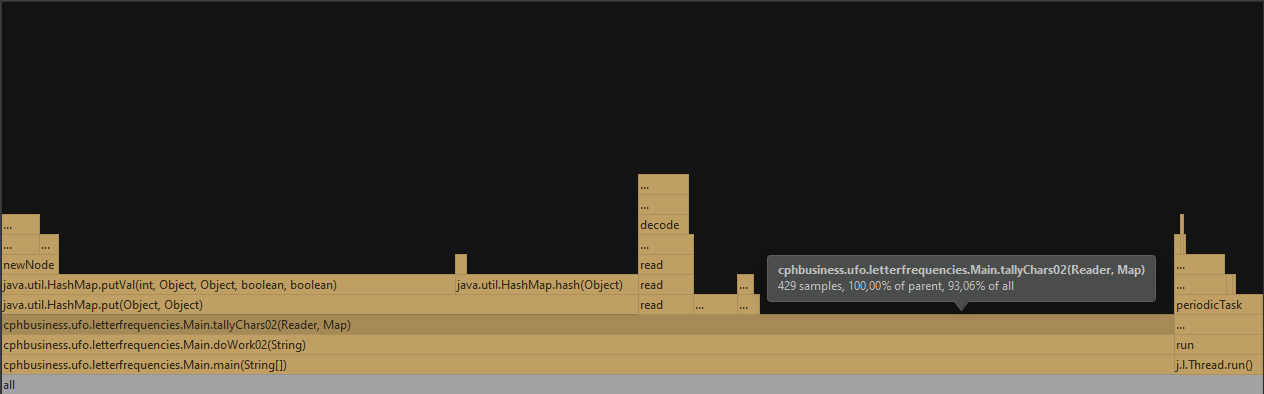
\includegraphics[width=\textwidth]{images/tallyChars02.PNG}
    \caption{Flammegraf med færre nestede kald fra tallyChars.}
    \label{fig:optimeret_fg}
\end{figure}
\paragraph{}
Koden er således klar til videre forædling. Vi opstiller her et par forslag som vil give yderligere forbedringer i kørselstiderne.
\begin{enumerate}
    \item Fjernelse af try-catch sætningen og istedet indsætte vha. getOrDefault-metoden på Map således:\begin{verbatim}
        freq.put((int)b, freq.getOrDefault((int)b, 0L) + 1)
    \end{verbatim}    
    \item Tråde til at indlæse parallelt.
    \item Alternativ datastruktur til HashMap (dog brud med kontrakt).
\end{enumerate}
\begin{figure}[htb]
    \centering
    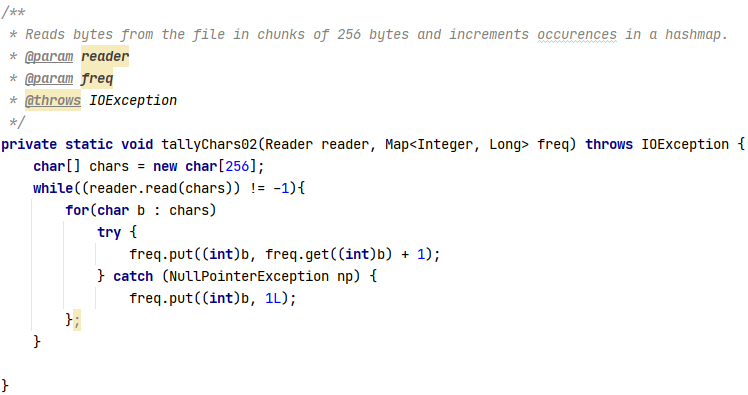
\includegraphics[width=\textwidth]{images/tallyChars02_code.PNG}
    \caption{Optimeret tallyChars metode.}
    \label{fig:optimeret}
\end{figure}
\end{document}
